%!TEX program = xelatex
% ****** Start of file TLGtheory.tex ******
%

\documentclass[%
 reprint,
%superscriptaddress,
groupedaddress,
%unsortedaddress,
%runinaddress,
%frontmatterverbose, 
%preprint,
showpacs,
%preprintnumbers,
%nofootinbib,
%nobibnotes,
%bibnotes,
 amsmath,amssymb,
 aps,
%pra,
prb,
%rmp,
%prstab,
%prstper,
%floatfix,
]{revtex4-1}

\usepackage{graphicx}% Include figure files
\usepackage{dcolumn}% Align table columns on decimal point
\usepackage{bm}% bold math
\usepackage{hyperref}% add hypertext capabilities
\usepackage{braket}

%\usepackage[mathlines]{lineno}% Enable numbering of text and display math
%\linenumbers\relax % Commence numbering lines

%\usepackage[showframe,%Uncomment any one of the following lines to test 
%scale=0.7, marginratio={1:1, 2:3}, ignoreall,% default settings
%text={7in,10in},centering,
%margin=1.5in,
%total={6.5in,8.75in}, top=1.2in, left=0.9in, includefoot,
%height=10in,a5paper,hmargin={3cm,0.8in},
%]{geometry}

% all eps files are in the figures 
\graphicspath{{figures/}}

\begin{document}

\preprint{APS/123-QED}

\title{Quantum information with continuous variables}% 
%\thanks{}%

\author{Wentao Jiang}%
 \email{jwt13@mails.tsinghua.edu.cn}

 \affiliation{%
2013011717, Department of Physics, Tsinghua University, Beijing 100084, China
}%

\date{\today}

\begin{abstract}
Quantum information and related techniques are well discussed during our class, however, many quantum variables are continuous, leading to the concept of continuous quantum informatioon processing. Universal quantum computation can be realized over continuous variables, which are as powerful as conventional qubits. This paper briefly summarizes the basic elements and operations for continuous-variable based quantum information and computation, and introduces some related protocols.
%\begin{description}
%\item[PACS numbers]
%May be entered using the \verb+\pacs{#1}+ command. 
%\end{description}
\end{abstract}
                             % Classification Scheme.
%\keywords{Suggested keywords}%Use showkeys class option if keyword
                              %display desired
\maketitle

% \tableofcontents

\section{Introduction} % (fold)
\label{sec:introduction}
	The field of quantum information mainly focused on the manipulation of discrete systems such as qubits, as in our QEEC class. However, many quantum variables are continuous, leading to the concept of continuous quantum information. Initially, the notions of quantum information processing with continuous variables were not well defined. Since the first experiment realization of quantum teleportation of optical fields, the strengths and weaknesses of continuous quantum information began to be understood and formulated. It turns out that universal quantum computation can be realized over continuous variables such as position, momentum or the quadratures of electromagnetic fields, and these continuous variables are as powerful as conventional qubits for any computation.

	Many qubit-based quantum information and computation protocols have their continuous-variable counterparts, and some of them are even easier to be experimentally realized comparing to discrete cases. The continuous-variable versions of these protocols are mostly based on Gaussian states and their manipulation through Gaussian operations, which are going to be defined later. This term paper is mainly based on a review,\cite{Braunstein2005} where I choose mostly related topics and techniques to be included in this paper.

	The paper is organized as follows. In Sec.~\ref{sec:continuous_variables_in_quantum_optics}, I briefly introduce quantum optics as a framework for continuous-variable based quantum information processing, where quantized electromagnetic modes, phase-space representation and Gaussian states are introduced. Section~\ref{sec:quantum_communication_and_computation_with_continuous_variables} describes several important quantum communication protocols in terms of continuous variables, most of which utilize continuous-variable entangled states, such as quantum teleportation, quantum error correction and universal quantum computation. Some concluding remarks are presented in Sec.~\ref{sec:conclusion}.
% section introduction (end)



\section{continuous variables in quantum optics} % (fold)
\label{sec:continuous_variables_in_quantum_optics}

	In quantum optics, the quantized electromagnetic modes correspond to quantum harmonic oscillators. The modes' quadratures play the roles of the oscillators' position and momentum operators, which are noncommuting Hermitian operators and obey Heisenberg uncertainty relation.

	In this section, I first summarize the definition and various relations of the field quadratures and phase-space representations of the state. Gaussian states and linear and nonlinear optical operations are then introduced, which are the basics for continuous-variable based quantum information.

	\subsection{Quadratures and representations} % (fold)
	\label{sub:quadratures_and_representations}
	
	\subsubsection{Quadratures} % (fold)
	\label{ssub:quadratures}
	
	% subsubsection quadratures (end)

		Let's start from the Hamiltonian of a quantum harmonic oscillator in terms of both creation/annihilation operators and ``position/momentum'' operators\footnote{I omit the hat distinguishing operators and numbers, when it can be deduced from the context.}
		\begin{equation}
			\label{eqns:ham_harmo_osci}
			H_k = \hbar \omega_k ( a^\dagger_k a_k +\frac{1}{2} )= \frac{1}{2} ( p_k^2 +\omega_k^2 x_k^2 ),
		\end{equation}
		where
		\begin{eqnarray}
			a_k &=& \frac{1}{\sqrt{2\hbar \omega_k}}(\omega_k x_k +ip_k),\\
			a_k^\dagger &=& \frac{1}{\sqrt{2\hbar \omega_k}}(\omega_k x_k -ip_k),\\
			x_k &=& \sqrt{\frac{\hbar}{2 \omega_k}} (a_k + a_k^\dagger),\\
			p_k &=& -i \sqrt{\frac{\hbar \omega_k}{2}}(a_k - a_k^\dagger),
		\end{eqnarray}
		and the commutation relations of these operators read
		\begin{eqnarray}
			[x_k,p_{k'}] &=& i \hbar \delta_{kk'},\\
			{}[a_k,a^{\dagger}_{k'}]&=& \delta_{kk'}.
		\end{eqnarray}
		It's easy to see that the position and the momentum are the real and imaginary part of the annihilation operator up to normalization factors, hence it's convenient to define the dimensionless pair of conjugate variables
		\begin{eqnarray}
			X_k = \sqrt{\frac{\omega_k}{2\hbar}}x_k &=& \mathrm{Re} (a_k) = \frac{1}{2} (a_k + a_k^\dagger),\\
			P_k = \frac{1}{\sqrt{2\hbar \omega_k}}p_k &=& \mathrm{Im} (a_k) = \frac{1}{2i} (a_k - a_k^\dagger),
		\end{eqnarray}
		and the commutation for $X_k,P_k$ is then $ [X_k, P_{k'}] = i \delta_{kk'}/2 $, which shows that we can treat $\hbar = 1/2$ in all usual relations with $x_k$ and $p_k$. For convenience, let's write $X_k, P_k$ as $x_k, p_k$ in the following and call them a conjugate pair of dimensionless quadratures of the field.

		In terms of these operators, a single mode of the electric field becomes
		\begin{eqnarray}
			 E_k(\bm r,t) &=& E_0 ( a_k e^{i(\bm k \cdot \bm r - \omega_k t)} +h.c.),\\
			&= &2E_0 [ x_k \cos ( \omega_k t - \bm k \cdot \bm r  ) \notag\\
			&&+ p_k \sin ( \omega_k t - \bm k \cdot \bm r  ) ],\\
			& =& 2E_0 [ x_k^{(\Theta)} \cos ( \omega_k t - \bm k \cdot \bm r -\Theta ) \notag\\
			&&+ p_k^{(\Theta)} \sin ( \omega_k t - \bm k \cdot \bm r -\Theta ) ],
		\end{eqnarray}
		where the more general quadratures are introduced
		\begin{eqnarray}
			x_k^{(\Theta)} &=& ( a_k e^{-i \Theta } + a_k^\dagger e^{ i \Theta} )/2,\\
			p_k^{(\Theta)} &=& ( a_k e^{-i \Theta } - a_k^\dagger e^{ i\Theta} )/2i.
		\end{eqnarray}

		\subsubsection{Phase-space representations} % (fold)
		\label{ssub:phase_space_representations}
			Sometimes it's convenient to use a classical-like probability distribution to picture the state in phase space, and one of the suitable candidates for this purpose is the Wigner function, which is proposed by Wigner\cite{PhysRev.40.749} and defined as
			\begin{equation}
			W(x,p) = \frac{2}{\pi} \int dy e^{4iyp}\bra{x-y} \rho \ket{x+y},
			\end{equation}
			where $x,p$ are the quadratures introduced before and $ \rho $ is the density operator. The probability distribution aspects of Wigner function are attributed to the following properties which resemble the normalization and marginal distributions
			\begin{eqnarray}
				\int W(\alpha)d^2 \alpha = 1, \int W dx = \bra p \rho \ket p, \int W dp = \bra x \rho \ket x, \notag
			\end{eqnarray}
			where $W (\alpha = x+ip) \equiv W(x,p) $ and $d^2 \alpha = d \mathrm{Re} \alpha d \mathrm{Im} \alpha = dxdp $ for short.

			Generally, there is a whole family of quasiprobability distributions to give a classical-like formulation of quantum optics, in which the Wigner function is perfectly suited to provide expectation values of quantities symmetric in $a$ and $a^\dagger $ such as the quadratures:
			\begin{equation}
			\label{eqn:quad_aver}
			\mathrm{Tr}[\rho \mathcal S(x^np^m)] = \int W(x,p)x^np^mdxdp,
			\end{equation}
			where $\mathcal S$ indicates symmetrization. Various nonclassical quantum states relevant to continuous-variable quantum communication can be formulated by means of the Wigner representation, including entanglement and nonlocality.			

		% subsubsection phase_space_representations (end)


	% subsection quadratures_and_representations (end)

	\subsection{Gaussian states and operations} % (fold)
	\label{sub:gaussian_states_and_operations}

		Gaussian states are defined by their corresponding Wigner functions, which are normalized Gaussian distributions of the form
		\begin{equation}
		W(\xi) = \frac{1}{ (2\pi)^N \sqrt{ \mathrm{det} V^{(N)} } } \exp \left\{ \frac{1}{2} \xi [V^{(N)}]^{-1} \xi^T \right\},
		\end{equation}
		where
		\begin{equation}
		\xi = (x_1,p_1,...,x_N,p_N) - (\bar x_1,\bar p_1,...,\bar x_N,\bar p_N),
		\end{equation}
		and the $2N\times 2N$ matrix $ V^{(N)} $'s elements are second moments according to Eq.~(\ref{eqn:quad_aver})
		\begin{equation}
		\mathrm{Tr} [ \rho \mathcal S ((\xi_i - \bar \xi_i)(\xi_j - \bar \xi_j) ) ] = \int W(\xi)\Delta\xi_i \Delta\xi_j d^{2N}\xi = V_{ij}^{(N)}.
		\end{equation}
		The last equality defines the correlation matrix for any quantum state. Hence for Gaussian states, the Wigner function is completely determined by the second moment correlation matrix.
		
		Viewing the Wigner function as a classical probability distribution over the $2N$-dimensional phase space, physical states require the correlation matrix to be real, symmetric and positive, and vice versa. In addition, the quadratures must also obey the commutation relation which can be written as
		\begin{equation}
		[\xi_k, \xi_l] = \frac{i}{2} \Lambda_{kl},
		\end{equation}
		where the $2N\times 2N$ matrix $ \Lambda $ is block diagonal with $2\times 2$ matrix $J = i \sigma_y $ as diagonal blocks.

		Now let's consider optical devices as operations on the field operators. Passive optical devices such as beam splitters and phase shifters conserve the photon number and correspond to linear transforms of the annihilation operator.

		A beam splitter can be considered as a four-port device relates the input and output annihilation operators in the Heisenberg picture and can be described by a unitary matrix in order to preserve the commutation relations. A general two-mode unitary transformation can be expressed by
		\begin{eqnarray}
			U(2) = \left (\begin{array}{cc}
				e^{-i(\phi +\delta)}\sin \theta & e^{-i \delta} \cos \theta \\
				e^{-i(\phi +\delta')}\cos \theta & -e^{-i \delta'} \sin \theta
			\end{array} \right ).
		\end{eqnarray}
		For a phase-free beam splitter, the input-output operators are related by		
		\begin{eqnarray}
			\left (\begin{array}{c}
				a_1'\\
				a_2'
			\end{array} \right ) = \left (\begin{array}{cc}
				\sin \theta &  \cos \theta \\
				\cos \theta &  -\sin \theta
			\end{array} \right )\left (\begin{array}{c}
				a_1\\
				a_2
			\end{array} \right ),
		\end{eqnarray}
		with $\sin \theta $ and $ \cos \theta $ the reflectivity and transmittance parameters. It's easy to see that a general unitary matrix can be realized by a series of phase shifts and phase-free beam-splitter rotations. By arranging 2-mode linear operations between different pairs of field operators, general $N\times N$ unitary linear transformations can be realized with linear optics\cite{PhysRevLett.73.58}
		\begin{equation}
		a_i' = \sum_j U_{ij} a_j
		\end{equation}

		The operations discussed above doesn't mix between the $a$'s and $a^\dagger$'s, where a nonlinear optical $ \chi^{(2)} $ interaction is required, for example in parametric amplification. The corresponded transformation generalizes to linear unitary Bogoliubov transformation
		\begin{equation}
		a_i' = \sum_j A_{ij}a_j + B_{ij} a^\dagger_j + \gamma_i,
		\end{equation}
		where $A$ and $B$ must satisfy $AB^T = (AB^T)^T$ and $ AA^\dagger = BB^\dagger + I $ in order to preserve bosonic commutation relations for $a_i'$.

		For a squeezing involving $ \chi^{(2)} $ interaction, the Hamiltonian is 
		\begin{equation}
		\label{eq:Ham_squeeze}
		H_{\mathrm{int}} = i\hbar \frac{\kappa}{2} a^{\dagger 2} e^{i \Theta} + h.c.,
		\end{equation}
		describing the amplification of mode $a$ at half the pump frequency. The resulting Heisenberg equation is $\dot a = \kappa a^\dagger $ and can be solved
		\begin{eqnarray}
		&a(t) = a(0) \cosh \kappa t + a^\dagger (0) \sinh \kappa t,\\
		&x(t) = e^{\kappa t} x(0), p(t) = e^{-\kappa t}p(0).
		\end{eqnarray}
		As a result, one quadrature is attenuated and the other amplified, the uncertainty of the $x$ quadrature grows at $e^{2 \kappa t} $ and the $p$ quadrature decreases at $ e^{- 2\kappa t} $, hence can lead to reduction of quantum fluctuations in one ovservable below the standard quantum limit. The unitary squeezing operator is just the unitary evolution of the above interaction Hamiltonian and is defined as
		\begin{equation}
		S(\zeta) = \exp \left (\frac{\zeta^*}{2} a^2 - \frac{\zeta}{2} a^{\dagger 2} \right ),
		\end{equation}
		where $\zeta=-r \exp(i \Theta), r=\kappa t $ is the squeezing parameter.

		Generally, all minimum uncertainty states are displaced squeezed states from vacuum,
		\begin{equation}
		\ket{\alpha, \zeta} = D(\alpha) S(\zeta) \ket{0},
		\end{equation}
		where the displacement operator $ D(\alpha) = \exp(\alpha a^\dagger - \alpha^* a ) $ and $ D^\dagger (\alpha) a D(\alpha) = a+\alpha $. The position wave function and Wigner function of $ \ket{\alpha,\zeta} $ is then
		\begin{eqnarray}
			&\psi = \left (\frac{2}{\pi} \right )^{1/4} e^{r/2}\exp[ -e^{2r} (x-x_{\alpha})^2 +2ip_{\alpha}x - ix_{\alpha}p_{\alpha} ], \notag\\
			& W = \frac{2}{\pi} \exp[ -2e^{2r} (x-x_{\alpha})^2 - 2e^{-2r} (p-p_{\alpha})^2 ].
		\end{eqnarray}

		Lastly, let's look at the process for producing a two-mode squeezed state which is a straight forward generalization of degenerate optical parametric amplification, the interaction Hamiltonian is
		\begin{equation}
		H_{\mathrm{int}} = i \hbar \kappa a_1^\dagger a_2^\dagger e^{i \Theta} + h.c.,
		\end{equation}
		and the solution
		\begin{eqnarray}
		\label{eqns:two_mode_squeezed}
			a_1 (t) &=& a_1 \cosh r + a_2^\dagger \sinh r,\notag\\
			a_2 (t) &=& a_2 \cosh r + a_1^\dagger \sinh r.
		\end{eqnarray}
		These modes are entangled and exhibit quantum correlations between the quadratures. It's important to note that the two-mode squeezed state above can also be obtained from two equally squeezed state (one squeezed in $x$ and another in $p$) by combining them at a 50:50 beam splitter, after which the two output modes will be in two-mode squeezed state. The derivation is straight forward in the Heisenberg representation.

		Now we have almost all building blocks for continuous-variable based quantum communication protocols, where the essential ingredient of most protocols is continuous-variable entanglement. For universal quantum computation, higher nonlinear process is required and is introduced in Sec.~\ref{sub:universal_quantum_computation}.

	% subsection gaussian_states_and_operations (end)

% section continuous_variables_in_quantum_optics (end)


\section{quantum communication and computation with continuous variables} % (fold)
\label{sec:quantum_communication_and_computation_with_continuous_variables}

	In this section I briefly introduce the continuous version of entanglement and other quantum communication and computation protocols with continuous variables.

	\subsection{Continuous-variable entanglement} % (fold)
	\label{sub:continuous_variable_entanglement}
		Although entanglement is always mentioned with discrete variables such as qubits, it's originally formulated by continuous variables. In the famous EPR paper,\cite{PhysRev.47.777} they considered the position function $ \psi(x_1,x_2) = C \delta(x_1-x_2-u) $ which describes perfectly correlated positions $(x_1-x_2=u)$ and momenta $ (p_1+p_2=0) $ but is however unphysical, with a vanishing normalization constant. Hopefully the state can be approximated by two-mode squeezed state with Wigner function
		\begin{eqnarray}
		W(\xi) &=& \frac{4}{\pi} \exp \big \{ -e^{-2r} [ (x_1+x_2)^2+(p_1-p_2)^2 ] \notag \\
		&& -e^{2r}[ (x_1-x_2)^2+(p_1+p_2)^2] \big \},
		\end{eqnarray}
		where the positions and momenta are correlated to some finite extent, and the Wigner function approaches $C \delta(x_1-x_2) \delta(p_1+p_2) $ when $r \rightarrow \infty $. By writing the state in Fock basis, it can be shown that the two modes are also quantum correlated in photon number and phase.\cite{Braunstein2005}

		The two-mode squeezed vacuum state is the quantum optical representative for bipartite continuous-variable entanglement. For general bipartite pure states, the necessary and sufficient condition for entanglement can be summarized by
		\begin{eqnarray}
			\text{entangled} &\Leftrightarrow& \text{Schmidt rank}>1, \notag\\
			\text{entangled} &\Leftrightarrow& \text{partial von Neumann entropy}>0, \notag \\
			\text{entangled} &\Leftrightarrow& \text{violations of local realism}. \notag
		\end{eqnarray}

		For mixed bipartite states, the definition of entanglement is generalized as nonseparability of the total density operator, namely, a two-party system is in a separable state iff its total density operator can be written as a sum of products of density operators of sub systems,
		\begin{equation}
		\label{eqn:two_mix_separable}
		\rho_{12} = \sum_i \eta_i \rho_{i,1}\otimes \rho_{i,2}.
		\end{equation}
		
		It is nontrivial whether a givendensity operator is separable or not, hence several practical criteria are proposed for testing the separability. One sufficient condition for inseparability is ``negative partial transpose''(npt) proposed by Peres.\cite{PhysRevLett.77.1413} For a separable state as in Eq.~(\ref{eqn:two_mix_separable}), the density operator after a partial transposition $\rho_{12}' = \sum_i \rho_{i,1}^T \otimes \rho_{i,2} $ is still a legitimate density operator. Hence it's a necessary condition for a separable state and one negative eigenvalue of $ \rho_{12}' $ is a sufficient condition for inseparability, but unfortunately not necessary except for specific classes of states.

		For discrete case, the partial transpose operation is straight forward. For continuous variable case, it's equivalent to sign change of the momentum operators: partial transpose is equivalent to complex conjugate due to the Hermiticity of the density operator, which is then equivalent to time reversal and hence sign change of the momentum.

		For bipartite Gaussian states with arbituarily many modes at each side, the inseparability problem is in principle solved via a finite number of iterations, proposed by Giedke, Kraus, \textit{et al.}\cite{PhysRevLett.87.167904} For bipartite two-mode states, sufficient criteria are proposed by different approaches\cite{PhysRevLett.84.2722,PhysRevLett.84.2726} and are also necessary for Gaussian states. Lastly, the inseparability criteria mentioned above are fulfilled	by the two-mode squeezed vacuum state as in Eq.~(\ref{eqns:two_mode_squeezed}) for any nonzero squeezing.
	
	% subsection continuous_variable_entanglement (end)

	\subsection{Quantum teleportation} % (fold)
	\label{sub:quantum_teleportation}

		Quantum teleportation with discrete variable is described in our class, where Alice and Bob share an entangled qubit pair. By measuring Alice's two qubits with respect to Bell states and sending results to Bob, the teleportation is realized.

		
		\begin{figure}[!h]
			\centering
			%width can be changed
			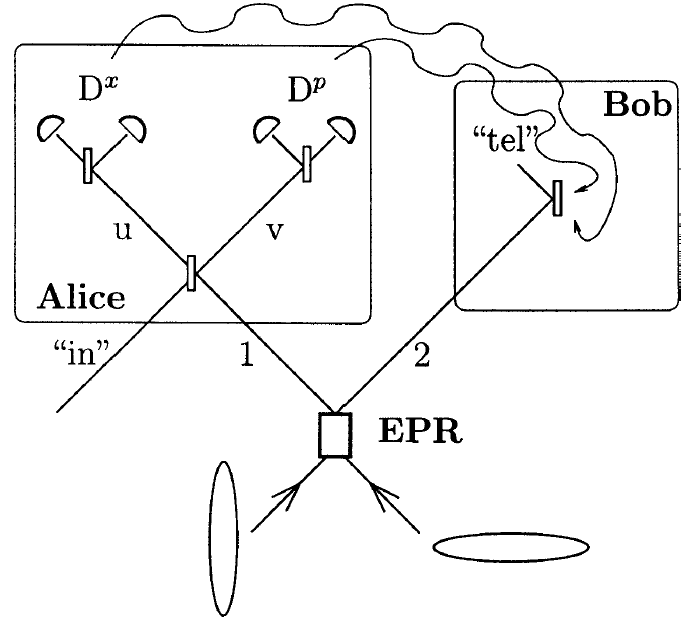
\includegraphics[width=2in]{fig1_teleport.png}
			\caption{Teleportation of a single mode of an electromagnetic field}
			\label{pic:teleport}
		\end{figure}

		For simplicity, let's consider teleportation of a single mode of the electromagnetic field with a shared two-mode squeezed state as the entangled source. As depicted in Fig.~\ref{pic:teleport}, the two-mode squeezed state is sent to Alice and Bob respectively. Alice then couple the entangled state with her input mode at a beamsplitter. The Bell detection on $x$ and $p$ quadratures are carried out on the beamsplitter output and results sent to Bob via classical channels.

		The mode to teleport is denoted by subscript ``in'' and the shared entangled two-mode squeezed state ``1'' and ``2''. After the beamsplitter, the output modes are given by
		\begin{eqnarray}
		\label{eqns:tele_BSoutput}
			x_u &=& (x_{in}-x_1)/\sqrt2, p_u = (p_{in} - p_1)/\sqrt2, \notag \\
			x_v &=& (x_{in} + x_1)/\sqrt2, p_v = (p_{in} +p_1)/\sqrt2.
		\end{eqnarray}
		Combining Eqs.~(\ref{eqns:tele_BSoutput}) with Eqs.~(\ref{eqns:two_mode_squeezed}), Bob's mode 2 can be written as
		\begin{eqnarray}
		x_2 &=& x_{in} - \sqrt2 e^{-r} x_2^{(0)} -\sqrt2 x_u,\notag\\
		p_2 &=& p_{in} + \sqrt2 e^{-r} p_1^{(0)} - \sqrt2 p_v,
		\end{eqnarray}
		where $r$ is the squeezing parameter. After receiving Alice's measurement results of $x_u$ and $p_v $, Bob can displace his mode,
		\begin{eqnarray}
		x_{tel} &=& x_2 + \sqrt2 x_u = x_{in} - \sqrt2 e^{-r} x_2^{(0)},\notag\\
		p_{tel} &=& p_2 + \sqrt2 p_v = p_{in} + \sqrt2 e^{-r} p_1^{(0)}.
		\end{eqnarray}
		Hence for infinite squeezing $r\rightarrow \infty$, perfect teleportation of the input mode can be realized.
		
	
	% subsection quantum_teleportation (end)

	\subsection{Dense coding} % (fold)
	\label{sub:dense_coding}

		The average information in an alphabet $A$ is given by $ I(A) =-\sum_a p_a \ln p_a $, where $p_a $ is the probability of symbol $a$. The mutual information in a pair of alphabets $A$ and $B$ is
		\begin{equation}
		I(A:B)=I(A)+I(B)-I(A,B)=\sum_{a,b} p_{ab}\ln \frac{p_{ab}}{p_a p_b}.
		\end{equation}
		Based on the mutual information, the channel capacity can be defined as
		\begin{equation}
		C = \max_{\{ p_a \}} I(A:B) = \max_{\{ p_a \}} \sum_{ab}p_{b|a} p_a \ln \frac{p_{b|a}}{p_b} ,
		\end{equation}
		where the channel is characterized by conditional probabilities $ p_{b|a} $. For continuous-variable channel which has an infinite-dimensional Hilbert space, some constraint must be adopted to get a finite capacity. The canonical constraint is that the mean number of quanta per usage has an upper bound $ \braket{n} = \bar n $. Then the max capacity corresponds to a thermal distribution for number states alphabet\cite{PhysRevLett.70.363} and
		\begin{equation}
		\label{eqn:classical_capacity}
		C = (1+\bar n)\ln (1+\bar n)\approx 1+\ln \bar n.
		\end{equation}

		In dense coding, Alice and Bob communicate via two channels one of which is a shared two-mode squeezed state and may be run off-peak. The entangled channel is not modulated and can be sent at any time, which is classically not possible. For a specific case where Alice displaces her mode and sends the state to Bob, by carrying out a homodyne detection, the original displacement signal can be extracted ideally. The corresponded capacity is\cite{Braunstein2005}
		\begin{equation}
		C^{\text{dense}} = \ln(1+\bar n +\bar n^2)\sim4r,
		\end{equation}
		for optimized $\bar n$ and large squeeze. In contrast, classical communication via quantum states from Eq.~(\ref{eqn:classical_capacity}) gives $ C\sim 2r $, showing that dense-coding allows twice as much information to be encoded within a given state.
		
	% subsection dense_coding (end)

	\subsection{Quantum error correction} % (fold)
	\label{sub:quantum_error_correction}
		There are a lot of quantum error correction codes and related theories for discrete variables, such as the well-known Shor's 9-qubit code, where 9 qubits are used to encode one logical qubit which can recover any one-bit error. For continuous variable, a similar nine-wave-packet code exists\cite{PhysRevLett.80.4084,nature.10.1038.27850} and corrects any one-wavepacket error.

		In the nine-wave-packet code, a position eigenstate $\ket x$ is encoded of the form
		\begin{eqnarray}
		\ket{x_{\text{encode}}} &=& \frac{1}{\pi^{3/2}} \int dwdydz \notag\\
		&& e^{2ix(w+y+z)}\ket{w,w,w,y,y,y,z,z,z},
		\end{eqnarray}
		which can be generated entirely using linear optics from $\ket{x_{\text{init}}} = \ket{x,0,0,0,0,0,0,0,0} $ with only nine channels and eight beam-splitters.\cite{nature.10.1038.27850} For no error, the inverted encoding gives the original state and all auxiliary wavepackets recover to zero position. If one of the wavepackets suffers from noise, inverted encoding yields a non-zero `syndrome' indicating the type and size of the error, which can be translated to a pure linear displacement as an appropriate remedy.
		
		Another usage of quantum error correcting codes over continuous variables is that states of a finite-dimensional system can be encoded into an infinite-dimensional Hilbert space of a continuous-variable system to fight against decoherence.\cite{PhysRevA.64.012310}
		
	% subsection quantum_error_correction (end)

	\subsection{Universal quantum computation} % (fold)
	\label{sub:universal_quantum_computation}

		For quantum computation with the amplitudes of electromagnetic field, it can be shown that a universal quantum computer might be constructed using linear optics, squeezers and at least one nonlinear optical elements such as the Kerr effect.

		Quantum computation over continuous variables seems hopeless at first sight because even a single continuous variable requires an infinite number of parameters to define, hence cannot be approximated by any finite number of quantum operations. On the other hand, it's possible to define universal quantum computation over certain subclasses of transformations, such as Hamiltonians that are polynomial functions of continuous-variable operators. If a finite number of applications of operators from a set of continuous quantum operators can generate a specific set of transformations, thenthe set of operators is termed universal for this set of transformations. The set of transformations to consider here corresponds to Hamiltonians that are arbituary polynomial functions of dimensionless operators $x$ and $p$.

		Let's first consider Hamiltonians $H=\pm x$ and $\pm p$. In Heisenberg picture, applying $x$ for time $t$ results in $x \rightarrow x, p \rightarrow p - t/2 $ and similarly $x\rightarrow x+t/2,p\rightarrow p $ for $p $. One might ask whether we are able to generate other forms of Hamiltonian if we already have $x$ and $p$, such as linear combination of $x$ and $p$. The answer is true for linear combination, and there is a general statement\cite{Deutsch669}: if one can apply a set of Hamiltonians $\{\pm H_i \} $, any Hamiltonian that is a linear combination of Hamiltonians of the form $\pm i[H_i,H_j],\pm[H_i,[H_j,H_k] ],... $ can be constructed and no other Hamiltonians. For example,
		\begin{equation}
		e^{-iA \delta t} e^{-i B \delta t} e^{i A \delta t} e^{ i B \delta t}=e^{[A,B] \delta t^2} + O(\delta t^3).
		\end{equation}
		As a result, any Hamiltonian $ax+by+c$ can be generated from $\pm x,\pm p$.

		For phase shift in linear optics, the Hamiltonian is $H = x^2 +p^2 $ and it's easy to verify the application of this Hamiltonian for time $t$ yields $x \rightarrow x\cos t -p\sin t, y\rightarrow p\cos t+x\sin t	$. The squeezing operation in Eq.~(\ref{eq:Ham_squeeze}) is described by $S = xp+px$ and gives $ x\rightarrow e^t x, p \rightarrow e^{-t} p $. $x$, $p$, $H$ and $S$ generate any Hamiltonian quadratic in $x$ and $p$ and no higher order. In order to construct higher-order Hamiltonian, at least one nonlinear operators are required, such as the Kerr Hamiltonian $H^2=(x^2+p^2)^2$. Commuting $H^2$ with the other four operators generates third-order polynomials. An inductive proof can show that arbituary Hermitian polynomials of $x$ and $p$ can be constructed when $H^2$ is added. Observe that
		\begin{eqnarray}
		[x^2, x^{M-n}p^n] &=& nix^{M-n+1} p^{n-1}/2 + \text{lower-order terms}, \notag\\
		{}[p^2,x^{M-n}p^n] &=& -(M-n)ix^{M-n-1}p^{n+1}/2 +\text{lower-order},\notag \\
		{}[x^3,x^np^m] &=& 3mix^{n+2}p^{m-1}/2 +\text{lower-order},\notag\\
		{}[p^3,x^np^m] &=& 3nix^{n-1}p^{m+2}/2 +\text{lower-order},\notag
		\end{eqnarray}
		which means we can generate any monomial of order $M+1$ can be constructed from monomials of order $M$. As a result, one can construct polynomials of arbitrary order in $x$ and $p$ to any desired degree of accuracy. Any higher-order Hamiltonian suffices to fulfill the goal of generating arbituary polynomial Hamiltonian of a single continuous variable.

		For multiple variables, if we can apply two-mode squeeze Hamiltonian $B_{ij} =x_ip_j-p_ix_j $, together with the above mentioned single variable operators, arbituary Hermitian polynomials of the set of continuous variables can be constructed. Hence the main result is: simple linear operations on continuous variables, together with any nonlinear operation and any interaction between variables, suffice to enact to an arbitrary degree of accuracy Hamiltonian operators that are arbitrary Hermitian polynomials of the set of continuous variables.
		
		
	% subsection universal_quantum_computation (end)


% section quantum_communication_and_computation_with_continuous_variables (end)



\section{conclusion} % (fold)
\label{sec:conclusion}
	In this paper, I briefly introduced the notion of continuous quantum variable based on quadratures of electromagnetic fields. Gaussian states and related operations are exploited to generated squeezed vacuum states and two-mode squeezed states, which show quantum correlation and are the crucial elements of many continuous-variable protocols.

	Continuous-variable entanglement is presented and several inseparability criteria mentioned. Quantum teleportation and dense coding is formulated using entangled states. Similar to Shor's nine qubit quantum error correction code, a nine-wave-packet code is introduced, which is able to correct any one-wavepacket error. Lastly, universal quantum computation with continuous variables is discussed, showing a small finite set of operators suffice to accomplish specific class of quantum computation.
	
% section conclusion (end)

\begin{acknowledgments}
	Thank teacher Zeng and the TA for this semester's QEEC class. In addition, the book (Ref.~\onlinecite{Zeng2015}) and the slices have been very helpful.
\end{acknowledgments}

\nocite{*}

\bibliographystyle{apsrev4-1}
\bibliography{QEEC}% Produces the bibliography via BibTeX.

\end{document}
%
% ****** End of file apssamp.tex ******
